\documentclass[sigconf]{acmart}

\usepackage{graphicx}
\usepackage{hyperref}
\usepackage{todonotes}

\usepackage{endfloat}
\renewcommand{\efloatseparator}{\mbox{}} % no new page between figures

\usepackage{booktabs} % For formal tables

\settopmatter{printacmref=false} % Removes citation information below abstract
\renewcommand\footnotetextcopyrightpermission[1]{} % removes footnote with conference information in first column
\pagestyle{plain} % removes running headers

\newcommand{\TODO}[1]{\todo[inline]{#1}}

\begin{document}
\title{Unsupervised Learning For Detecting Fake Online Reviews}


\author{Syam Sundar Herle}
\affiliation{%
  \institution{Indiana University}
  \city{Bloomington} 
  \state{IN} 
  \postcode{47408}
  \country{USA}}
\email{syampara@iu.edu}


\begin{abstract}
Nowadays decision making done by organization and individuals highly weighted on online reviews, social media opinions of any product or services. There is lot of valuable information available online, on which if proper mining technique is used we can reveal hidden values which are way useful to day to day life decision making. Given the usefulness of online data, individuals and group of people have started to take advantage of those data to boost up their business or products or creating an biased competition in market and this type of individuals and group of people create an opinion spamming system. Opinionated spamming are spams created by spammers to benefit their business fame or profit by giving biased reviews of product or service. Mechanism to detect these spammers or spam created by these spammers is an urgent need as we our technology has raised to new standard and raise in the rate of accessibility to online due to available technology. Here we are going to propose a such mechanism to detect fake review with help of an unsupervised machine learning model, which is trained using opinion mining of Natural Language Processing (NLP). Opinion mining is an art of extracting opinions of author, speaker or writer from their written text or spoken words, opinion mining is done by employing Natural Language Processing ,text analysis, Artificial Intelligence. 

\end{abstract}

\keywords{HID 219, Opinionated Spamming, Artificial Intelligence, Opinion Mining, Machine Learning, Natural Language Processing (NLP)}

\maketitle

\section{Introduction}

Usually the sentiment analysis can be defined as classifying a piece of written text into positive,negative or neutral state. This is also known as opinion analysis as it derives the opinion of the author. Said that, now a days, user's and consumers write reviews, opinions on online for a product or service given to them. The growth of web and internet has enabled user or consumers to communicate among each other and write up more reviews about products and has made the web more subjective and opinionated. As a result, huge amount of data in the form of texts are available from online which are rich in information, which are users review and opinion about products and service delivered to them. Which in turn can be used by the product owners to meet the consumer needs and demands, and provide quality products and identify the issues in products and much more. Unbiased and independent reviews about a product are the main decision making entity usually used by peoples while purchasing a product. 
Opinion mining is usually employed for the knowledge retrieval from textual contents such as review and comments. Opinion mining results the the textual content in one of the three categories namely positive, negative and neutral. Positive opinion are good in yielding good financial gains and fame and good business for product owners. On the other hand negative reviews helps in identifying the issues of the products, having said that some people usually write fake reviews to boost their financial gain or discredit their competitive product. These type of reviews are known as opinion spammers. In the following we will learn about sentiment analysis in detail and we will walk through some of the achievement done in detecting fake review and opinion spammers and we will propose our unsupervised learning model.

\section{Overview of Sentiment Analysis}

As defined earlier, sentiment analysis or opinion mining is the study of peoples opinion, attitude and emotion towards a product or any other entity. Usually the sentiment analysis is done on the textual contents like reviews of product, twitter tweets and comments in public blog about any entities. The overview of the sentiment analysis can be seen the Figure \ref{f:SA}.

\begin{figure}[!ht]
  \centering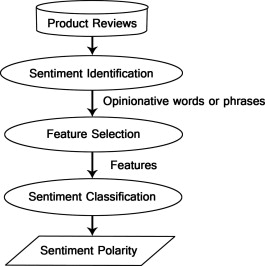
\includegraphics[width=\columnwidth]{images/sa.jpg}
  \caption{Sentiment Analysis on product review \cite{sentianalysis}}\label{f:SA}
\end{figure}

Overall, sentiment analysis is considered to be a classification process, which is done by three different types, the first one is being document sentiment analysis where the texts of documents are used to classify the opinion of the whole documents, the other type is sentence sentiment analysis where the texts of the sentence is used to classify the opinion of the sentence and third one is being aspect-level sentiment analysis where sentence or document are classified with respect to specific aspects of entity (product or service). 
\subsection{Data}
In the first step of Sentiment Analysis, data are collected from online, the preferred data are reviews of product as these data are textual contents and unstructured and rich in information. These data are important in the sentiment analysis as the business owner can make use of the analysis of these data (review of product) to learn about users opinion about the product. The social media network are one of the good and important source of these types of data as users and consumers interact and post review of the products from their own accounts. 

The second important step is identifying the words or phrases which are useful in the forming the opinion in the sentence or document based on the type of sentiment analysis we intend to do as told in earlier paragraph. The following sub-section describes the next each steps in sentiment analysis in detail.

\subsection{Feature Selection}
The very important step in sentiment analysis is extracting features needed for the analysis, some of the feature selection used are,\textbf{Bag of Words and Frequency} in which a vector of binary is used as features, the binary vector comprises of 1 and 0 based on the presence of words in the document or sentence and forming a bag of binary vector for all words. The other weight used in these type of feature is the frequency of the words in the sentence or document. 

The next type of features used in sentiment analysis is \textbf{Part Of Speech} where the part of speech tagger is used to create features, in this method grammatical context tag of the words in sentence or document is used, these types features helps to find the emotion of the author from his or her texts.

The other features employed are \textbf{Opinion words and Negations} where features are built based upon the words which determines the words as bad or good and negation features gives overall appearance of the negative words in sentence or document.
\subsubsection{Feature Selection Methods} 
Here we can see some of the methods employed to extract and select features to perform sentiment analysis on the sentence or document. Usually feature selection can be done by two types of methods, \textbf{Lexicon-based} \cite{lexi} method and \textbf{Statistical-based} \cite{statis} method. The first method needs human annotation like bag of words (BOW) \cite{lexi} but the second method is usually is fully automated. Some of the statistical methods used in feature selection are given as follows,
\subsubsection*{Chi-Square $\tilde{\chi}^2$} : In chi-square test, the correlation between the term and categories is checked. According to \cite{sentianalysis} Consider n documents in any collection, and $p_{i}(w)$ be the conditional probability of class $i$ for document which contains the word $w$. and $P_{i}$ be the global fraction of document containing the class $i$, and $F(w)$ be the global fraction of document containing the word $w$. So the chi-square can be calculated as given in \cite{sentianalysis},
$$\tilde{\chi}^2 = \frac{n.F(w)^{2}.(p_{i}(w)-P_{i})^2}{F(w).(1-F(w)).P_{i}.(1-P_{i})}$$

The chi-square gives weights value for the words in the document and these value can be used as features for the sentiment analysis.

\subsubsection*{Information Gain} : In this method features are created based on the ranks of Information Gain entropy grouped in descending order. "The information gain usually measures the amount of information in bits about the class prediction, it also measures the expected reduction in entropy" \cite{Duch2006}.

\subsubsection*{Point-Wise Mutual Information} : This model provides mutual information between feature and classes, and this is derived from the information theory. According to \cite{sentianalysis} the point-wise mutual information, $M_i(w)$ is the information between the word $w$ and class $i$. So, we in laymen terms , the 
PMI \cite{sentianalysis} is the ratio between expected co-occurrence of class $i$ and $w$ which is given by $F(w).p_i(w)$ and the true occurrence which is given by $F(w).P_i$, so the PMI is defined as,
$$M_i(w) = log\bigg(\frac{F(w).P_i}{F(w).p_i(w)}\bigg)$$

The word $w$ is positive correlated to class $i$ if the value of $M_i(w)$ is greater than 0. Comparing with chi-square, PMI is not normalized value and hence for most of the feature selection chi-square is used.

\subsection{Classification Technique}

The classification technique employed for the sentiment analysis can be done by three approaches, Machine Learning approach, Lexicon based approach and use of both ML and Lexicon approach. In this sub-section we will walk through some of the techniques followed in all the three approaches.

\subsubsection{Machine Learning Approach}
Typical machine learning algorithms or predictive models are used in this approach, typically the ML approach can be divided into two models, Supervised learning and Unsupervised learning. 
\subsubsection*{Supervised Learning} : In supervised learning, a model is trained with the help of the labeled training data set and evaluated on the unseen data set which are known as test data set. After evaluating the test data classification accuracy are calculated to know how good the trained model is in classifying. Some of the supervised learning model used in sentiment analysis for classification techniques are,
\begin{itemize}
    \item Naive Bayes classifier : The Naive-Bayes is one of the probabilistic classifier, which works based on probabilities value to determine class. According to \cite{sentianalysis} the Naive-Bayes model predicts the posterior probability of a class to which the document belongs to, based on distribution of words in the document. For a given features it calculates the probability of the label assuming all the features $(f_i-f_n)$ are independent to each other, the Naive-Bayes follows the following equation to classify the class to which the document belongs to given the features, the features are generated by the Bag Of Words model.
    \begin{equation*}
        P(label/features) = \frac{P(label)*P(f_{1}/label)*.*P(f_{n}/label)}{P(features)}
    \end{equation*}
    As the above equation assumes the naive assumption of independence and uses Bayes theorem, it is known as the Naive-Bayes model.
    
    \item Support Vector Machine : Support Vector Machine model works based on the linear separation of the features which separates features in the search space to separate them based upon their classes, SVM is one of the linear classifier used in supervised learning ML approach. In SVM, the features are transformed to a higher dimensional state space and hyperplanes are used to separate the features, hyperplanes are determined by support vectors, which are features closer to the decision boundary of the separation of the features. For $n$ class of class the model needs $n-1$ support vectors. "SVM can construct a nonlinear decision surface in the original feature space by mapping the data instances non-linearly to an inner product space where the classes can be separated linearly with a hyperplane" \cite{sentianalysis}. In the case opinion mining, the classification are two positive and negative and hence one support vector is needed to do sentiment analysis.
    
    \item Neural Network : Neural Network (NN) consists of many basic unit which are known as neurons, the word frequencies in a document $X_i$ is given as input to the neuron, which has certain weights $A$ to compute probabilities values $P_i$ which is a product of $X_i*A$, the probability values acts as a linear function $f(.)$. So the linear function is given by,
    \begin{equation*}
    f(.) = X_i*A    
    \end{equation*}
    For the classification problem the linear function predicts the class label for the input $X_i$. The more the layer of neuron the better the output prediction will be, hence Multilayer Neural Network is employed in the classification problem if the number of class is more than 2.
\end{itemize}

\subsubsection*{Unsupervised Learning}
In the case of unsupervised learning, we will create a model to classify the classes of the data, the model is made to learn from the unlabelled data. In the case of sentiment analysis, analysis is done based on the similarity of the text and clustering them. Some of the unsupervised learning approach used in sentiment analysis are, 
\begin{itemize}
    \item LDA :  Latent Dirichlet allocation model is generative statistic model, Xianghua and Guo \cite{XIANGHUA2013186} used LDA model to automatically discover the aspects discussed in Chinese social reviews and also the sentiments expressed in different aspects.
    \item k-means : k-means employ metric to calculate distance between features created by bag of words (BOW) to cluster the words. 
    \item Cosine Similarity: Based on cosine similarity of word vectors, the textual content are grouped. In the case of any detection mechanism the target variables are detected by visualizing the pattern formed by the target variables.

\end{itemize}

\section{Related Work}

In this section we are going to walk through some of related work in detecting fake reviews, in \cite{1} an unexpected review pattern was studied and in \cite{} an graph based model was studied to investigate the fake review detection. An supervised learning model was introduced in \cite{2} to study the detection of individual fake reviewers, by using duplicate reviews and near duplicate reviews as ground truth of fake review to classify the unseen reviews. As the labeled set was duplicate, the learning model was niot able to give good accuracy of predicting the fake reviewers. In \cite{1} product review data was used to build a supervised learning model, the features for the model was based on the review text and product information to distinguish between duplicate review and non duplicate reviews. In \cite{http://ieeexplore.ieee.org.proxyiub.uits.iu.edu/document/7726174/} fake review detection was done using the semantic and emotional model. In \cite{http://ieeexplore.ieee.org.proxyiub.uits.iu.edu/document/7822945/} a semi-structured learning model was used to detect online deceptive detection, for this they used sentiment polarity and part of speech of words with linguistic inquiry word count  to create a supervised model to learn to classify the fake reviews and used the same features given to the model to create an unsupervised model to classify fake reviews.

In \cite{http://ieeexplore.ieee.org.proxyiub.uits.iu.edu/stamp/stamp.jsp?tp=&arnumber=8026965} a semi supervised learning model was created in two phases, where in first phase a Naive Bayes classifier was trained with the labeled data set and in the semi supervised phase they incorporated they created an unsupervised learning model with the features of Naive Bayes and used EM algorithm to create a SGD to classify the fake reviews.  In this work they used product review data from Amazon product review and used FIM \cite{http://ieeexplore.ieee.org.proxyiub.uits.iu.edu/stamp/stamp.jsp?tp=&arnumber=8026965} to train the Naive Bayes in the phase 1 and used precision, recall and F1-score as performance metric to evaluate SGD.

For sentiment analysis, sentiment lexicon or opinion lexicon is needed to classify the text into the different groups which is positive,negative and neutral. One of the method using the opinion lexicon to do sentiment analysis on the text is meta-level feature \cite{BRAVOMARQUEZ201486}. In this method, sum on the positive word and sum on the negative word are calculated to classify the text into specific opinion. As this method is manual in nature, a method based on genetic algorithm is proposed in \cite{KESHAVARZ20171} ALGA : Adaptive Lexicon learning using Genetic Algorithm, which creates opinion lexicon dynamically and addresses the manual problem and optimization problems in meta-level feature. But in case if big data is used in sentiment analysis then, ALGA results will be bad, in order to address this, big data analytic technology need to be incorporated \cite{bigdatainsenti}. According to \cite{bigdatainsenti} the runtime problem in \cite{KESHAVARZ20171} is tackled by using MapReduce framework of Big Data, by dividing the jobs of calculating scores of positive lexical and negative lexical into independent tasks and run them in parallel on large-scale cluster. In MapReduce framework program, the input data are partitioned into independent set and in Map program the independent set are compiled to produce key and value tuples where key is the word and value is the frequency of the respective word and in the Reduce program the tuples are combined. By doing so, the computational time ALGA \cite{KESHAVARZ20171} is reduced. 

Using bigger data usually requires more memory and also more computation time. In order to address this issue, Apache Hadoop \cite{hadoopsenti} was used to store data in efficient manner. Hadoop consists of HDFS file system and MapReduce engine that manages the data storage blocks. HDFS consists of Namenode and Datanode \cite{hadoopsenti} where the Namenode manages all the Datanode and as said earlier MapReduce deals the parallel processing of the data with the help of the master node and slave node. For various classification and clustering problem on the huge data, Apache Mahout \cite{hadoopsenti} is used. For the evaluation process in \cite{hadoopsenti} Apache Mahout splits the data set into training set and test set. The training set is used to train the classifier.

For spotting fake reviews via collective positive-unlabeled learning \cite{http://ieeexplore.ieee.org.proxyiub.uits.iu.edu/stamp/stamp.jsp?tp=&arnumber=7023420} they used a Iterative Classification Algorithm ICA \cite{same} on reviews data to create features for the Multi-typed Heterogeneous Collective classification algorithm for the classification problem. As this was an classification problem they used labeled and unlabeled data set.

\section{Proposed Work}
The main goal of our proposed work is to detect opinion spammers, if we are going to employ a supervised learning as discussed in related work section we will be needing a labeled data set. But most of the data sources available on online are unstructured data without any labels for the fake reviews, in \cite{2} they used duplicate review as ground truth for classifying the fake reviews but the accuracy of proposed system in \cite{2} will be very low. If we want to create a labeled data set then we have to create a labeled data set Amazon Mechanical Trunk \cite{} or segregate opinion groups manually. Even though both the process of creating labeled data set are easy to implement, they have their own disadvantages. Both mentioned process are expensive and industrious to implement. 

As there is a scarcity of labeled data set available for reviews, we will propose a novel unsupervised learning to detect fake review on the non-labeled data set using cosine similarity approach. In this section we will explain more about the data and feature generation technique which was employed and about main algorithm of the proposed work.

\subsection{Data}
For the proposed work we have used data from the Yelp Dataset Challenge which includes data from the Phoenix, Las Vegas, Madison, Waterloo and Edinburgh, with 42,153 businesses and 1,125,458 reviews. Yelp uses its own filtering algorithm to remove fake data set, but we will try to examine the effectiveness of their algorithm by our proposed novel method.





\section{CONCLUSION}
Although still in its infancy, blockchain has the potential to be just as transformative as TCP/IP. Early and potential applications in healthcare and supply chain suggest that blockchain is indeed moving along the path of technology adoption. Because blockchain is a low-cost solution for supply chain management and provides security and transparency, it can be used for digital data and communication to overall the distribution of controlled substances such as opioids but this model has yet to be tested. But the computation and infrastructure cost for the entire model is low and should be tested to develop a proof of concept system that leverages blockchain to more securely distribute prescription opioids. A prototype model of blockchain can be developed which emulates the current structure of a pharmaceutical supply chain. Such a model can be vital to test out the flaws of blockchain and how to accurately tailor it to the specific use case.  

\begin{acks}
The authors would like to thank Dr. Gregor von Laszewski for his support and suggestions to write this paper.
\end{acks}

\bibliographystyle{ACM-Reference-Format}
\bibliography{report} 

\appendix

\section{Issues}

\DONE{Example of done item: Once you fix an item, change TODO to DONE}

\subsection{Assignment Submission Issues}

    \TODO{Do not make changes to your paper during grading, when your repository should be frozen.}

\subsection{Uncaught Bibliography Errors}

    \TODO{Missing bibliography file generated by JabRef}
    \TODO{Bibtex labels cannot have any spaces, \_ or \& in it}
    \TODO{Citations in text showing as [?]: this means either your report.bib is not up-to-date or there is a spelling error in the label of the item you want to cite, either in report.bib or in report.tex}

\subsection{Formatting}

    \TODO{Incorrect number of keywords or HID and i523 not included in the keywords}
    \TODO{Other formatting issues}

\subsection{Writing Errors}

    \TODO{Errors in title, e.g. capitalization}
    \TODO{Spelling errors}
    \TODO{Are you using {\em a} and {\em the} properly?}
    \TODO{Do not use phrases such as {\em shown in the Figure below}. Instead, use {\em as shown in Figure 3}, when referring to the 3rd figure}
    \TODO{Do not use the word {\em I} instead use {\em we} even if you are the sole author}
    \TODO{Do not use the phrase {\em In this paper/report we show} instead use {\em We show}. It is not important if this is a paper or a report and does not need to be mentioned}
    \TODO{If you want to say {\em and} do not use {\em \&} but use the word {\em and}}
    \TODO{Use a space after . , : }
    \TODO{When using a section command, the section title is not written in all-caps as format does this for you}\begin{verbatim}\section{Introduction} and NOT \section{INTRODUCTION} \end{verbatim}

\subsection{Citation Issues and Plagiarism}

    \TODO{It is your responsibility to make sure no plagiarism occurs. The instructions and resources were given in the class}
    \TODO{Claims made without citations provided}
    \TODO{Need to paraphrase long quotations (whole sentences or longer)}
    \TODO{Need to quote directly cited material}

\subsection{Character Errors}

    \TODO{Erroneous use of quotation marks, i.e. use ``quotes'' , instead of " "}
    \TODO{To emphasize a word, use {\em emphasize} and not ``quote''}
    \TODO{When using the characters \& \# \% \_  put a backslash before them so that they show up correctly}
    \TODO{Pasting and copying from the Web often results in non-ASCII characters to be used in your text, please remove them and replace accordingly. This is the case for quotes, dashes and all the other special characters.}
    \TODO{If you see a figure and not a figure in text you copied from a text that has the fi combined as a single character}

\subsection{Structural Issues}

    \TODO{Acknowledgement section missing}
    \TODO{Incorrect README file}
    \TODO{In case of a class and if you do a multi-author paper, you need to add an appendix describing who did what in the paper}
    \TODO{The paper has less than 2 pages of text, i.e. excluding images, tables and figures}
    \TODO{The paper has more than 6 pages of text, i.e. excluding images, tables and figures}
    \TODO{Do not artificially inflate your paper if you are below the page limit}

\subsection{Details about the Figures and Tables}

    \TODO{Capitalization errors in referring to captions, e.g. Figure 1, Table 2}
    \TODO{Do use {\em label} and {\em ref} to automatically create figure numbers}
    \TODO{Wrong placement of figure caption. They should be on the bottom of the figure}
    \TODO{Wrong placement of table caption. They should be on the top of the table}
    \TODO{Images submitted incorrectly. They should be in native format, e.g. .graffle, .pptx, .png, .jpg}
    \TODO{Do not submit eps images. Instead, convert them to PDF}

    \TODO{The image files must be in a single directory named "images"}
    \TODO{In case there is a powerpoint in the submission, the image must be exported as PDF}
    \TODO{Make the figures large enough so we can read the details. If needed make the figure over two columns}
    \TODO{Do not worry about the figure placement if they are at a different location than you think. Figures are allowed to float. For this class, you should place all figures at the end of the report.}
    \TODO{In case you copied a figure from another paper you need to ask for copyright permission. In case of a class paper, you must include a reference to the original in the caption}
    \TODO{Remove any figure that is not referred to explicitly in the text (As shown in Figure ..)}
    \TODO{Do not use textwidth as a parameter for includegraphics}
    \TODO{Figures should be reasonably sized and often you just need to
  add columnwidth} e.g. \begin{verbatim}/includegraphics[width=\columnwidth]{images/myimage.pdf}\end{verbatim}

re

\end{document}
